\section{Feature Extraction}

\subsection{Term Frequency}

When classifying text files a logical first feature to take a look at is Term-Frequency (TF).
TF just counts for each token the number of time it appears in the text file.
However, there are different ways to approach this. 
Instead of using a single word as a token it is possible to take any number of words that appear sequentially  as a feature, this is called an n-gram.

\subsection{Term Frequency- Inverse Document Frequency}

A way to counter the problems TF has we can use Term Frequency-Inverse Document Frequency (TF-IDF).
Instead of just looking at how frequently a term is in the document we also look at how common it is accross all cocuments.
In that way, common terms accross all documents become less important features, while terms that are special to a document become more important.

We explored for TF-IDF at different ranges of n-gram options to determine what gave the best results, see Figure~\ref{fig:ngram}.
Interestingly a unigram (1-gram) gave the best results when using an out-of-the-box logistic regressor. 

\begin{figure*}[ht!]
    \centering
    \subfloat[F1-score for different ngram ranges\label{fig:ngram-f1}]{%
        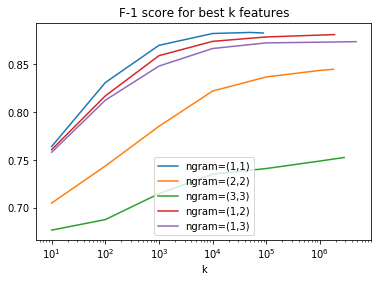
\includegraphics[width=0.3\linewidth]{figures/ngram_range/f1-score.png}}
    \hfill
    \subfloat[Precision-score for different ngram ranges\label{fig:ngram-precision}]{%
        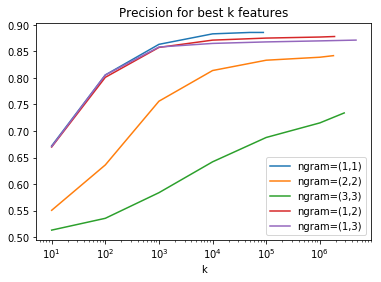
\includegraphics[width=0.3\linewidth]{figures/ngram_range/precision-score.png}}
        \hfill
    \subfloat[Recall-score for different ngram ranges\label{fig:ngram-recall}]{%
        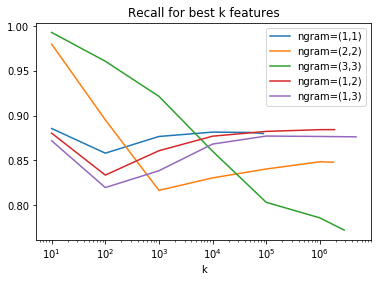
\includegraphics[width=0.3\linewidth]{figures/ngram_range/recall-score.png}}
  \caption{Ngram}
  \label{fig:ngram} 
\end{figure*}

\subsection{Sentiment Analysis}
The previous two features TF and TF-IDF are focussing on frequency of the words that appear in a document, but it doesn't make any distinction between the words.
The third feature we are looking at focussing exactly on this problem. Instead of looking at individual words, we can look at each review on its own and determine its sentiment.
Achieving this is done by applying \textit{Valence Aware Dictionary and Sentiment Reasoner}, also known as VADER, on each review.
For each review we then get a tuple with four values: positive, compound, neutral, or negative. These features can then be used to train a classifier.


\subsection{Comparison}

When the three different set of features are compared we can see clearly that TF-IDF is performing best out of the three, closely followed by TF, and on a distance Sentiment analysis using VADER.
It is interesting that VADER, did not perform better. It shows that it is very complex to summarize a text down to just four values.
It still performs considerably better than random, but there is a big gap in performance between TF and VADER.

\begin{table}[ht!]
    \centering
    \caption{Results for different features using an out-of-the-box logistic regressor\label{tab:features-comp}}
    \begin{tabular}{ l| S[table-format=1.3] |S[table-format=1.3] |S[table-format=1.3] }
    \hline
        \bf{Feature} & \bf{F1-measure} & \bf{Precision} & \bf{Recall} \\
    \hline
        TF & 0.868 & 0.876 & 0.859 \\ 
        TF-IDF & 0.886 & 0.883 & 0.889 \\
        VADER & 0.719 & 0.716 & 0.721 \\
        \hline
    \end{tabular}
\end{table}

\subsection{Feature Extraction Pipeline}
Based on the results that we found for each feature, we present our feature extraction pipeline in Figure~\ref{fig:feature-selection}.
We chose to use TF-IDF over TF and VADER because of the clearly better performance it gives.
For ngram-range we chose a range of (1,1), meaning we will only use unigrams.
Unigrams seemded to give the best performance as can be seen in Figure~\ref{fig:ngram}.

\begin{figure}[ht!]
    \setlength{\unitlength}{0.14in}
    \centering
    \begin{picture}(20,10)
    \put(2,4){\framebox(5,3){\footnotesize{TF}}}
    \put(8,4){\framebox(5,3){\footnotesize{TF-IDF}}}
    \put(14,4){\framebox(5,3){\footnotesize{KBest}}}
    \put(1,1.5){\framebox(19,8){}}
    
    \put(0,5.5){\vector(1,0){2}}
    \put(7,5.5){\vector(1,0){1}}
    \put(19,5.5){\vector(1,0){2}}
    
    \end{picture}
    \caption{Pipeline for the Feature Selection}
    \label{fig:feature-selection}
\end{figure}
